\section{Introduction}

%\paragraph{Motivation}

Simultaneously imaging large populations of neurons using calcium sensors is becoming increasingly popular.
%, both in vitro  \cite{ImagingManual} and in vivo \cite{NagayamaChen07, GobelHelmchen07, LuoSvoboda08}, especially as the signal-to-noise-ratio (SNR) of genetic sensors continues to improve \cite{GaraschukKonnerth07, MankGriesbeck08, WallaceHasan08}. 
Whereas the data from these experiments are movies of time-varying fluorescence signals, the desired signal is typically the spike trains of the observable neurons.  %Importantly, Because somatic calcium concentration has a relatively simple relationship to spikes, in theory, one could infer the most likely spike train of each neuron, given the fluorescence data.  
% 
%\paragraph{Limitations of calcium imaging}
% 
Unfortunately, finding the most likely spike train is a challenging computational task, due to poor signal-to-noise (SNR), poor temporal resolution, unknown parameters, and computational intractability.
%for a number of reasons.  First, the signal-to-noise ratio (SNR) is often low, especially as one increases the image field and frame rate.  Second, fluorescence data typically has a low temporal resolution.  Third, to find the most likely spike train for a given fluorescence signal, one would have to search over all possible spike trains, a search that would take far too long, in practice.  
% 
%\paragraph{Computational tools as important as experimental tools}
% 
One is therefore effectively forced to find an approximately most likely spike train, or guess that the inferred spike train is most likely (but not really be sure).  %The precise details of these approximations, however, are crucial, especially as one approaches shot-noise limited data. For in vitro studies, one often uses 1-photon imaging --- either confocal or widefield --- in which case the number of photons per neuron is a function of magnification and frame rate (obviously, other parameters, such as number of sensors per neuron, are also important, but typically more difficult to control).  To maximize the amount of information one can extract from such preparations, one should increase the frame rate and image field until achieving the shot noise limited regime, assuming one has an inference algorithm that can operate in such a scenario.  For in vivo studies, 2-photon laser scanning microscopy is currently the method of choice, for which the SNR is relatively low,  because the dwell time per pixel is (frame duration)/($\#$ of pixels in frame).  To circumvent the low SNR for in vivo studies, some groups use long integration times (e.g., \cite{OhkiReid06}), whereas others use small image fields (e.g., \cite{KerrHelmchen07}).  One would prefer to neither sacrifice temporal resolution nor number of observable neurons, to get sufficient signal quality to perform reliable inference.  Therefore, it is of the utmost importance to extract as much information as possible from the signal; especially if one is asking quantitative questions about the statistics of the spike trains from the observable neurons --- either spontaneously or in relation to some sensorimotor stimulus or other spiking neurons.
%
%\paragraph{Previous approaches}

A number of groups have therefore proposed algorithms to infer spike trains from calcium fluorescence data.  For instance, Greenberg et al. \cite{GreenbergKerr08} developed a novel template matching algorithm. %, which performed well on their data, but is not particularly computationally efficient
Holekamp et al. \cite{HolekampHoly08} took a very different strategy, by performing the optimal linear deconvolution (i.e., the Wiener filter) on the fluorescence data.  This approach is natural from a signal processing standpoint, but does not utilize the knowledge that spikes are always positive.  Previously, a sequential Monte Carlo method to efficiently compute the approximate probability of a spike in each image frame, given the entire fluorescence time series, was proposed \cite{VogelsteinPaninski09}.  While effective, that approach is not suitable for online analyses of populations of neurons, as the computations run in approximately real-time per neuron (i.e., analyzing one minute of data requires about one minute of computational time on a standard laptop computer), and real-time for a whole population of neurons would be desirable.


The present work therefore takes a somewhat different approach.  It starts by first carefully considering the statistics of typical data-sets, and then writing down a generative model that accurately relates spiking to observations. Unfortunately, inferring the most likely spike train given this model is computationally intractable.  Making some well-justified approximations leads to an algorithm that infers the approximately most likely spike train, given the fluorescence data.  This algorithm has a few particularly noteworthy features, relative to other approaches.  First, spikes are assumed to be positive.  This assumption often improves filtering results when the underlying signal has this property \cite{LeeSeung99, HuysPaninski06}.  Second, the algorithm is extremely fast: it can process a calcium trace from 50,000 images in about one second on a standard laptop computer. In fact, filtering the signals for an entire population of about $100$ neurons runs \emph{faster} than real time. This speed facilitates using this filter online, as observations are being collected. In addition to these two features, the model may be generalized in a number of ways, including incorporating spatial filtering of the raw movie. The efficacy of the proposed filter is demonstrated on several real data-sets, suggesting this algorithm is a powerful and robust tool for online spike train inference.  The code (which is a simple Matlab script) is available from the authors upon request.







\section{Methods} \label{sec:methods}

As described above, to develop an algorithm to approximate the most likely spike train given fluorescence data, the statistics of typical data-sets are analyzed.  Starting with an in vitro experiment, for which the SNR is relatively high, an appropriate generative model is built (Section \ref{sec:model}).  Given this model, a goal can formalized (Section \ref{sec:goal}).  And given this goal, an approximately optimal inference algorithm is derived (Section \ref{sec:inf}) .  This algorithm depends on a number of unknown parameters, which can be estimated directly from the fluorescence observations (Secion \ref{sec:learn}).  The effective signal-to-noise ratio (SNR) of the fluorescence trace can be potentially improved by spatially filtering the movie (Section \ref{sec:spatial}), even when multiple neurons are within a region-of-interest (ROI) (Section \ref{sec:methods:overlapping}).  


\subsection{Data driven generative model} \label{sec:model}

Figure \ref{fig:in_vitro_ex} shows a typical in vitro, epifluorescence data-set (see Section \ref{sec:exp} for data collection details).  The top panel shows a field-of-view, including 3 neurons, two of which are patched.  To build the model, a region-of-interest (ROI) is defined,  which is this case is the circled neuron.  Given the ROI, all the pixel intensities of each frame can be averaged, to get a one-dimensional fluorescence time-series, as shown in the bottom left panel (black line).  By patching onto this neuron, the spike train can also be directly observed (black bars). Previous work suggests that this fluorescence signal might be well characterized by convolving the spike train with an exponential, and adding noise \cite{ImagingManual}.  This model is confirmed by convolving the true spike train with an exponential (gray line, bottom left panel), and then looking at the distribution of the residuals.  The bottom right panel shows a histogram of the residuals (black line), and the best fit Gaussian distribution (gray line).


\begin{figure}[h!]
\centering 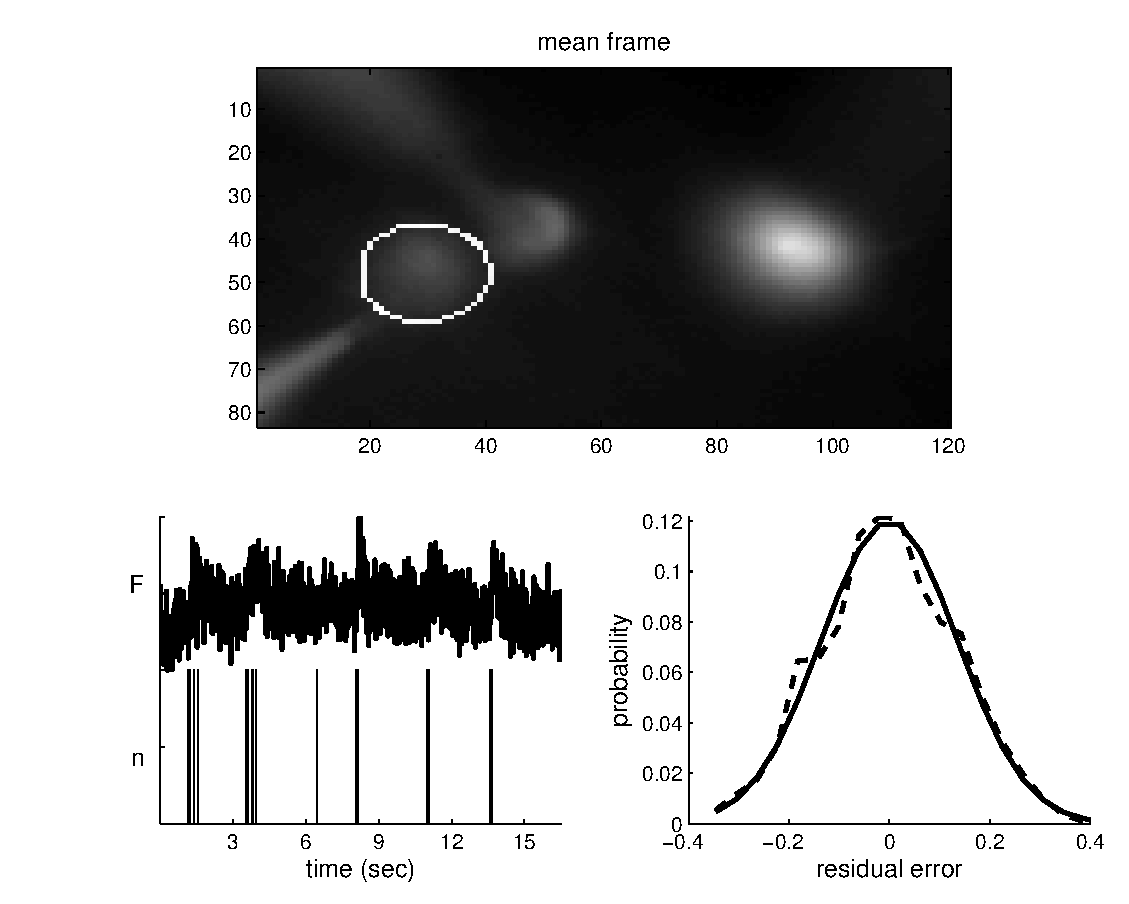
\includegraphics[width=.9\linewidth]{/Users/joshyv/Research/oopsi/fast-oopsi/figs/in_vitro_ex}
\caption[data-based model]{A typical in vitro data-set suggests that a reasonable first order model may be constructed by convolving the spike train with an exponential, and adding Gaussian noise. Top panel: the average (over frames) of a typical field-of-view.  Bottom left: spike train (black bars), convolved with an exponential (gray line), superimposed on the one-dimensional fluorescence time series (black line).  Bottom right: a histogram of the residual error between the gray and black lines from the bottom left panel (black line), and the best fit Gaussian (gray line).} \label{fig:in_vitro_ex}
\end{figure}

The above observations may be formalized as follows. Assume there is a one-dimensional fluorescence trace, $\bF=(F_1, \ldots, F_T)$ from a neuron.  At time $t$, the fluorescence measurement, $F_t$ is a linear-Gaussian function of the intracellular calcium concentration at that time, $C_t$:

\begin{align} \label{eq:F}
F_t &= \alpha (C_t + \beta) + \sig \varepsilon_t, \qquad \varepsilon_t \overset{iid}{\sim} \mN(0,1).
\end{align}

\noindent The scale, $\alpha$, absorbs all experimental variables impacting the scale of the signal, including number of sensors within the cell, photons per calcium ion, amplification of imaging system, etc.  Similarly, the offset, $\beta$, absorbs baseline calcium concentration of the cell, background fluorescence of the fluorophore, imaging system offset, etc.  The standard deviation, $\sig$, results from calcium fluctuations independent of spiking activity, fluorescence fluctuations independent of calcium, and imaging noise. The noise at each time, $\varepsilon_t$, is independently and identically distributed according to a standard normal distribution (i.e., Gaussian with zero mean and unit variance). 

Then, assuming that the intracellular calcium concentration, $C_t$, jumps by $A$ $\mu$M after each spike, and subsequently decays back down to $C_b$ $\mu$M with time constant, $\tau$, yields:

\begin{align} \label{eq:C}
C_{t+\Del} = (1- \Del/\tau ) C_t + C_b + A n_t
\end{align}

\noindent where $\Del$ is the time step size --- which is the frame duration, or $1/$(frame rate) --- and $n_t$ indicates the number of times the neuron spiked in frame $t$. %, and $\gam=1-\Del/\tau$. \footnote{This follows from writing \eqref{eq:C} as $\tau \frac{C_t - C_{t-1}}{\Del} = -C_{t-1} + n_t$.} 
Note that because $C_t$ and $F_t$ are linearly related to one another, the fluorescence scale, $\alpha$, and calcium scale, $A$, are not separable and therefore not identifiable.  In other words, we can set either to unity without loss of generality, as the other can absorb the scale entirely.  Similarly, the fluorescence offset, $\beta$, and calcium baseline, $C_b$ are not separable, so either can be set to zero without loss of generality.  Finally, letting $\gam=(1-\Del/\tau)$, Eq. \eqref{eq:C} can be rewritten: $C_{t+\Del}=\gam C_t + n_t$. Note that given this simplification,  $C_t$ does not refer to absolute intracellular concentration of calcium, but rather, a relative measure (but see \cite{VogelsteinPaninski09} for a more general model).  The gray line in the bottom left panel of Figure \ref{fig:in_vitro_ex} corresponds to the putative $\bC$ of the observed neuron.  

To complete the ``generative model'' (i.e., a model from which simulations cab be generated), the distribution from which spikes are sampled must be defined.  Perhaps the simplest first order description of spike trains is that at each time, spikes are sampled according to a Poisson distribution with some rate:

\begin{align} \label{eq:n}
	n_t \overset{iid}{\sim} \text{Poisson}(\lam \Del)
\end{align}

\noindent where $\lam \Del$ is the expected firing rate, and $\Del$ is included to ensure that the expected firing rate is independent of the frame rate.  Thus, Eqs. \eqref{eq:F} -- \eqref{eq:n} complete the generative model.  






\subsection{Goal} \label{sec:goal}

Given the above model, the goal is to find the maximum \emph{a posteriori} (MAP) spike train, i.e., the most likely spike train, $\hbn$,  given the fluorescence measurements, $\bF$. Formally:

\begin{align} \label{eq:nhat1} 
\hbn &=  \anx P[\bn | \bF], 
\end{align}

\noindent where $P[\bn | \bF]$ is the posterior probability of a spike train, $\bn$, given the fluorescent trace, $\bF$, and $n_t$ is constrained to be an integer ($\mathbb{N}_0=\{0,1,2,\ldots\}$).  From Bayes' Rule, the posterior can be rewritten:

\begin{align} \label{eq:bayes}
P[\bn | \bF] = \frac{P[\bn, \bF]}{P[\bF]} = \frac{1}{P[\bF]} P[\bF | \bn] P[\bn],
\end{align}

\noindent where $P[\bF]$ is the evidence of the data; $P[\bF | \bn]$ is the likelihood of a observing a particular fluorescence trace $\bF$, given the spike train $\bn$, and $P[\bn]$ is the prior probability of a spike train.  Plugging Eq. \eqref{eq:bayes} into Eq. \eqref{eq:nhat1}, yields:

\begin{align} \label{eq:nhat2} 
\hbn &=  \anx \frac{1}{P[\bF]} P[\bF | \bn] P[\bn] =  \anx  P[\bF | \bn] P[\bn],
\end{align}

\noindent where the second equality follows because $P[\bF]$ merely scales the results, but does not change the relative quality of various spike trains.  Fortunately, both $P[\bF | \bn]$ and $P[\bn]$ are available from the above model:

\begin{subequations} \label{eq:post1}
\begin{align}
P[\bF | \bn]&= P[\bF | \bC] 	= \prod_t P[F_t | C_t], \label{eq:lik1} \\ 
P[\bn] 		&= \prod_t P[n_t], \label{eq:prior1}
\end{align}
\end{subequations}

\noindent where the first equality in Eq. \eqref{eq:lik1} follows because $\bC$ is deterministic given $\bn$, and the second equality follows from Eq. \eqref{eq:F}. Further, Eq. \eqref{eq:prior1} follows from the Poisson distribution assumption, Eq. \eqref{eq:n}.  Both $P[F_t | C_t]$ and $P[n_t]$ can be written explicitly:

\begin{subequations} \label{eq:post2}
\begin{align}
P[F_t | C_t] &= \mN(F_t; \alpha(C_t+\beta),\sig^2), \label{eq:lik2} \\
P[n_t] &= \text{Poisson}(n_t; \lam \Del). \label{eq:prior2} 
\end{align}
\end{subequations}

\noindent where $\mN(x;\mu,\sig^2)$ indicates $x$ has a Gaussian distribution with mean $\mu$ and variance $\sig^2$ and Poisson$(x;k)$ indicates that $x$ has a Poisson distribution with rate $k$, and both equations follow from the above model.  Now, plugging Eq. \eqref{eq:post2} back into \eqref{eq:post1}, and plugging that result into Eq. \eqref{eq:nhat2}, yields:

\begin{subequations}  \label{eq:obj}
\begin{align}
\hbn 	&= \anx \prod_t \frac{1}{\sqrt{2 \pi \sig^2}} \left(-\frac{1}{2}\frac{(F_t - \alpha (C_t + \beta))^2}{\sig^2}\right) \frac{\text{e}^{-\lam\Del} (\lam\Del)^{n_t}}{n_t!}
\label{eq:obj1}\\ &= \anx  \sum_t \bigg( -\frac{1}{2 \sig^2}(F_t - \alpha(C_t + \beta))^2  -  n_t \log \lam \Del + \log n_t! \bigg), \label{eq:logobj1}
\end{align} 
\end{subequations}

\noindent where the second equality follows from taking the logarithm of the right-hand-side.  Unfortunately, solving Eq. \eqref{eq:logobj1} exactly is computationally intractable, as it requires a nonlinear search over an infinite number of  possible spike trains.  The search space could be restricted by imposing an upper bound, $k$, on the number of spikes within a frame.  However, in that case, the computational complexity scales \emph{exponentially} with the number of image frames --- i.e., the number of computations required would scale with $k^T$ --- which for pragmatic reasons is intractable.  Thus, Eq. \eqref{eq:obj} is approximated by modifying Eq. \eqref{eq:n}, replacing the Poisson distribution with an exponential distribution.  The advantage of this approximation is that the optimization problem becomes log-concave, meaning that any gradient ascent method guarantees achieving the global maximum (because there are no local maxima, other than the single global maximum).  The disadvantage, however, is that the integer constraint is lost, i.e., the answer could include ``partial'' spikes.  This disadvantage can be remedied by thresholding, or by considering the magnitude of a partial spike as the probability of a spike occurring in that time bin.  




\subsection{Inference} \label{sec:inf}

The goal here is to develop an algorithm to efficiently approximate $\hbn$, the most likely spike train, given the fluorescence trace. By letting Poisson$(n_t; \lam\Del) \approx$ Exponential$(n_t; \lam\Del)$, Eq. \eqref{eq:logobj1} becomes:

\begin{align} \label{eq:obj2}
\hbn &\approx \argmax_{n_t>0 \, \forall t}  \sum_{t=1}^T \bigg( -\frac{1}{2 \sig^2}(F_t - \alpha(C_t + \beta))^2  - n_t \lam \Del \bigg) 
\end{align}

\noindent where the constraint on $n_t$ has been relaxed from  $n_t \in \mathbb{N}_0$ to $n_t \geq 0$ (since the exponential distribution can yield any non-negative number), and '$+$'sreplaced $\max$ with $\min$ because '$+$'s inverted the signs.  Note that replacing a Poisson with an exponential is a common approximation technique in the machine learning literature \cite{PaninskiWu09}, as the exponential distribution is the closest convex relaxation to its non-convex counterpart, the Poisson distribution. While this convex relaxation makes the problem tractable, the ``sharp'' threshold imposed by the non-negativity constraint prohibits the use of standard gradient ascent techniques \cite{CONV04}. This problem may be rectified by dropping the sharp threshold, and adding a barrier term, which must approach $-\infty$ as $n_t$ approaches zero (this approach is often called an ``interior-point'' method) \cite{CONV04}. Iteratively reducing the weight of the barrier term guarantees convergence to the correct solution \cite{CONV04}.  Thus, the goal is to efficiently solve:

\begin{align} \label{eq:eta}
\hbn_{\zzz} &= \argmax_{n_t \forall t}  \sum_{t=1}^T \left( -\frac{1}{2 \sig^2}(F_t - \alpha(C_t + \beta))^2  -  n_t  \lam \Del + \zzz \log(n_t) \right).
\end{align}

\noindent Iteratively solving for $\hbn_{\zzz}$ for $z$ going from $1$ down to nearly $0$,guarantees convergence to $\hbn$. Since spikes and calcium are related to one another via a simple linear transformation, namely, $n_t=C_t-\gam C_{t-1}$, Eq. \eqref{eq:eta} may be rewritten in terms of $\bC$:

\begin{align} 
\hbC_{\zzz} &= \argmax_{C_t - \gamma C_{t-1} \geq 0 \forall t} \sum_{t=1}^{T} \left( -\frac{1}{2 \sig^2} (F_t -\alpha (C_t + \beta))^2  - (C_t - \gamma C_{t-1}) \lam \Del + \zzz \log(C_t - \gamma C_{-1}) \right). \label{eq:eta2}
\end{align}

\noindent The concavity of Eq. \eqref{eq:eta2} facilitates utilizing any number of techniques guaranteed to find the global optimum.  The fact that the argument of Eq. \eqref{eq:eta2} is twice differentiable, allows for the use of the Newton-Raphson technique, which is typically more efficient than only incorporating the gradient \cite{CONV04}. First, rewrite Eq. \eqref{eq:eta2} in matrix notation.  Note that $\bM \bC = \bn$:

\begin{align} \label{eq:M}
\ve{M} \bC = %- \bb=
\begin{bmatrix}
1 & 0  & 0 & \cdots & \cdots \\
1 & -\gamma & 0 & \cdots & \cdots \\
0 & 1 & -\gamma & 0 & \cdots  \\
\vdots & \vdots & \vdots & \vdots & \vdots  \\
0 & 0 & 0 & 1 & -\gamma
\end{bmatrix}
\begin{bmatrix}
C_1 \\ C_2 \\ \vdots \\ \vdots \\ C_T  
\end{bmatrix}
= 
\begin{bmatrix}
n_1 \\ n_2 \\ \vdots \\ \vdots \\ n_T
\end{bmatrix}
= \bn
\end{align}

\noindent where $\ve{M} \in \mathbb{R}^{T \times T}$ is a bidiagonal matrix.  Then, leting $\ve{1}$ be a $T$ dimensional column vector and $\blam=\lam \Del \ve{1}\T$, yields: 

\begin{align} 
\hbC_{\zzz} 
&= \az  -\frac{1}{2 \sig^2} \norm{\bF - \alpha (\bC +\beta)}^2 - (\bM \bC )\T \blam  + \zzz \log(\bM \bC)\T\ve{1},  \label{eq:eta3}
\end{align}

\noindent where $\bM \bC \geq \ve{0}$ indicates that every element of $\bM \bC$ is greater than or equal to zero, $\T$ indicates transpose, and $\log(\cdot)$ indicates an element-wise logarithm. Now, when using Newton-Raphson to ascend a gradient, one iteratively computes both the gradient (first derivative), $\bg$ , and Hessian (second derivative), $\bH$, of the argument to be minimized, with respect to the variables of interest ($\bC_z$ here).  Then, the estimate is updated using $\bC_z \leftarrow \bC_z + s \bd$, where $s$ is the step size. Solving $\bH \bd = \bg$ provides $\bd$, the step direction.  The gradient and Hessian are given by:

\begin{subequations} \label{eq:NR}
\begin{align}
\ve{g} &= -\frac{\alpha}{\sig^2}(\bF -\alpha({\hbC\T}_{\zzz} + \beta)) + \ve{M}\T\blam - \zzz \ve{M}\T (\ve{M} \hbC_{\zzz})^{-1} \label{eq:g} \\
\ve{H} &= \frac{\alpha^2}{\sig^2} \ve{I} + \zzz \ve{M}\T (\ve{M} \hbC_{\zzz})^{-2} \ve{M} \label{eq:H}
\end{align}
\end{subequations}

\noindent where the exponents indicate element-wise operations. The step size, $s$, is found using ``backtracking linesearches'', which finds the maximal $s$ that decreases the likelihood and is between $0$ and $1$.

Typically, implementing Newton-Raphson requires inverting the Hessian, i.e., $\bd = \bH^{-1} \bg$, a computation that scales \emph{cubically} with $T$, i.e., requires approximately $T^3$ operations. Already, this would be a drastic improvement over the most efficient algorithm assuming Poisson spikes, which require $k^T$ operations (where $k$ is the maximum number of spikes per frame).  Here, because $\ve{M}$ is bidiagonal, the Hessian is tridiagonal, the solution may be found in approximately $T$ operations, via standard banded Gaussian elimination techniques (which can be implemented efficiently in Matlab using $\bH \backslash \bg$). In other words, the above approximation and inference algorithm reduces computations from \emph{exponential} time to \emph{linear} time. 





\subsection{Learning} \label{sec:learn}

In the above, the parameters governing the model, $\vth=\{\alpha, \beta, \sig, \tau, \lam\}$, were assumed to be known. An approximate expectation-maximization algorithm estimates the parameters from the data, by thaking the following steps: (i) initialize some estimate of the parameters, $\hbth$, then (ii) recursively compute $\hbn$ using those parameters and update $\hbth$ given $\hbn$, and (iii) stop recursing when some convergence criteria is met.  

\subsubsection{Initializing the parameters}

Because the above model is linear, the scale of $\bF$ is arbitrary, so $\alpha$ can be fixed at $1$ without loss of generality.  The offset, however, is relative but is not arbitrary.  Because spiking is assumed to be sparse, $\bF$ tends to be around baseline, $\beta$ is initialized to be the median of $\bF$, and $\sig$ is initialized as median absolute deviation of $\bF$, ie, $\sig=$median$_s$($|F_s-$median$(\bF)|$).  Because previous work has shown that results are somewhat robust to minor variations in $\tau$ \cite{YaksiFriedrich06}, $\tau$ is initialized at 1 sec.  Finally, $\lam$ is initialized at $1$ Hz, which is between typical baseline firing rates and evoked spike rate activity, for these data-sets.

\subsubsection{Estimating the parameters given $\widehat{\mathbf{n}}$}

In the typical expectation-maximization setting, one finds the parameters that maximize the expected value of the joint observed and hidden signals:

\begin{align} \label{eq:par1}
\hbth &= \argmax_{\bth} E_{P[\bF | \bC]} \log P[\bF, \bC | \bth].
\end{align}
In the above, however, those expected values are not computed, rather, only the MAP estimate of the spike train and calcium trace.  Therefore, Eq. \eqref{eq:par1} is approximated by simply maximizing the parameters given the MAP estimate:

\begin{align} \label{eq:par2}
\hbth &\approx \argmax_{\bth} P[\bF| \hbC; \bth] P[\hbn | \bth]
\end{align}

\noindent where $\hbC$ is determined using the above described inference algorithm. The approximation in \eqref{eq:par1} is good whenever the likelihood is very peaky, meaning that most of the mass is around the MAP sequence.\footnote{The approximation in \eqref{eq:par1} may be considered a first-order Laplace approximation}   The argument from the right-hand-side of Eq \eqref{eq:par1} may be expanded: 

\begin{align} \label{eq:par2}
P[\bF| \hbC; \bth] P[\hbn | \bth] &= \prod_t P[F_t | \hC_t; \beta,\sig]  P[\hn_t | \lam].
\end{align}

\noindent where $\alpha$ is not present because of the arbitrary scale term, and $\tau$ is not present because it is not separable from $\hbn$. $\beta$ is estimated using:

\begin{align}
	\hbeta &= \argmax_{\beta >0} \prod_t P[F_t | \hC_t; \beta,\sig] = \argmax_{\beta>0} \sum_t (F_t - (C_t + \beta))^2,
\end{align}

\noindent which is solved by letting $\hbeta=\langle \bF-\bC \rangle_t$, where $\langle \cdot \rangle_t$ indicates a mean over $t$.  $\sig$ is then the mean of the residuals, and $\hlam$ is the mean of $\hbn$. 

\subsubsection{Convergence criteria}

Iterations stop whenever (i) iteration number exceeds some upper bound, or (ii) relative change in likelihood does not exceed some lower bound.  In practice, parameters tend to converge after several iterations, given the above initialization. 


\subsection{Spatial filtering} \label{sec:spatial}

In the above, it was assumed that the raw movie of fluorescence measurements collected by the experimenter had undergone two stages of preprocessing.  First, the movie was segmented, to determine regions-of-interest (ROIs).  This yields a vector, $\vF_t=(F_{1,t}, \ldots, F_{N_p,t})$, corresponding to the fluorescence intensity at time $t$ for each of the $N_p$ pixels in the ROI.  Second, at each time $t$, that vector is projected into a scalar, yielding $F_t$, the assumed input.  In this section, the optimal projection is determined by considering a more general model:

\begin{align} \label{eq:bF}
F_{x,t} &= \alpha_x (C_{x,t} + \beta) +  \sig \vec{\varepsilon}_{x,t}, \qquad &\varepsilon_{x,t} \overset{iid}{\sim} \mathcal{N}(0,1)   
\end{align}

\noindent where $\alpha_x$ scales each pixel, from which some number of photons are contributed due to calcium fluctuations, $C_t$, and others due to baseline fluorescence, $\beta$.  Further, the noise is assumed to be both spatially and temporally white, with variance, $\sig^2$, in each pixel (an assumption that can be relaxed quite easily).  Performing inference in this more general model proceeds nearly identical as before. Rewriting n vector notation:

\begin{align} 
\hbC_{\zzz} 
&= \az  -\frac{1}{2 \sig^2} \norm{\vec{\bF} - \valpha (\bC\T +\beta\ve{1}\T)}^2 - (\bM \bC )\T \blam  + \zzz \log(\bM \bC)\T\ve{1},  \label{eq:eta4}\\
\ve{g} &= \frac{\valpha}{\sig^2}(\vbF -\valpha({\hbC\T}_{\zzz} + \beta)) - \ve{M}\T\blam + \zzz \ve{M}\T (\ve{M} \hbC_{\zzz})^{-1} \label{eq:g2} \\
\ve{H} &= -\frac{\valpha\T \valpha}{\sig^2} \ve{I} - \zzz \ve{M}\T (\ve{M} \hbC_{\zzz})^{-2} \ve{M} \label{eq:H2}
\end{align}

\noindent where $\vbF$ is an $N_p$ by $T$ element matrix, $\valpha$ is column vectors of length $N_p$, and $\bI$ is an $N_p \times N_p$ identity matrix.  Typically, the spatial filter, $\valpha$ is unknown, and therefore must be estimated from the data.  In practice, letting $\valpha=\langle \vbF \rangle_t$ was both effective and extremely efficient.




\subsection{Overlapping spatial filters} \label{sec:methods:overlapping}

In the above, the image was assumed to be segmented, such that only a single neuron was within each ROI.  However, segmentation is itself a difficult problem \cite{}.  Therefore, using a crude segmentation technique, that might not actually produce ROIs with only a single cell, and then building spatial filters for each neuron in the ROI, might be more efficient and improve SNR.  As before, this requires a minor modification to Eq.~\eqref{eq:bF}.  Specifically, letting the superscript $i$ index the $N_c$ neurons in this ROI, yields:  

\begin{align}
\vF_t &= \sum_{i=1}^{N_c}\valpha^i (C^i_t + \beta^i) +  \sig\vec{\varepsilon}_t, \qquad &\vec{\varepsilon}_t \overset{iid}{\sim} \mathcal{N}(\ve{0},\bI)   \\
C^i_t &= \gam^i C^i_{t-1} + n^i_t, & n^i_t \sim \text{Poisson}(n^i_t; \lam_i \Del)
\end{align}

\noindent where each neuron is implicitly assumed to be independent, and that each pixel is independent and identically distributed with variance $\sig^2$.  To perform inference in this more general model, let:

\begin{align} \label{eq:M2}
\bn &=  [n^1_1, n^2_1, \ldots, n^{N_c}_1, n^1_2, \ldots, n^{N_c}_T]\T \\
\bC &=  [C^1_1, C^2_1, \ldots, C^{N_c}_1, n^1_2, \ldots, C^{N_c}_T]\T \\
\ve{M} &= %- \bb=
\begin{bmatrix}
1 & 1 & 0 & 0 & \cdots & \cdots \\
1 & -\gam^1 & 1 & -\gam_2 & \ldots & 1 & -\gam_{N_c}  & 0 & \cdots \\
\vdots & \vdots & \vdots & \vdots & \vdots  \\
0 & 0 & 0 \ldots & 1 & -\gam^{N_c-1} & 1 & -\gam^{N_c}
\end{bmatrix}
\end{align} 

\noindent and proceed as above, making minor algorithmic adjustments to deal with dimensionality issues.  Since the parameters will be unknown, they must be estimated. Define $\balpha_x=[\alpha_x^1, \ldots, \alpha_x^{N_c}]\T$ and $\bbeta=[\beta^1, \ldots, \beta^{N_c}]\T$.  To initialize, let $\bbeta=\ve{0}$, and $\valpha^i$ be the $i^{th}$ principal component of $\vbF$.  Then, iterate the following two steps.  Given $\bbeta$, use a quadratic solver to update each $\balpha_x$ (eg, in Matlab, $\balpha_x = (\bC + \widetilde{\bbeta})\backslash \bF_x$, where $\widetilde{\bbeta}$ is $\bbeta$ reparameterized to be the same size as $\bC$).  Given this estimate of $\balpha_x$ for all $x$, update $\beta^i= \frac{1}{T}\sum_t (\vF_t / \valpha^i - C_t^i)$ for each $i$, where $/$ indicates an element-wise division.  In practice, iterating these two steps converged after several iterations, assuming enough spikes were present in the two neurons, and they were sufficiently uncorrelated.








\subsection{Experimental Methods} \label{sec:exp}

\subsubsection{Slice Preparation and Imaging}

All animal handling and experimentation was done according to the National Institutes of Health and local Institutional Animal Care and Use Committee guidelines. Somatosensory thalamocortical slices $400$ $\mu$m thick were prepared from C57BL/6 mice at age P14 as described \cite{MacLeanYuste05}. Neurons were filled with $50$ $\mu$M Fura $2$ pentapotassium salt (Invitrogen, Carlsbad, CA) through the recording pipette. Pipette solution contained $130$ K-methylsulfate, $2$ MgCl$_2$, $0.6$ EGTA, $10$ HEPES, $4$ ATP-Mg, and $0.3$ GTP-Tris, pH $7.2$ ($295$ mOsm).  After cells were fully loaded with dye, imaging was done by using a modified BX50-WI upright confocal microscope (Olympus, Melville, NY).  Image acquisition was performed with the C9100-12 CCD camera from Hamamatsu Photonics (Shizuoka, Japan) with arclamp illumination at $385$ nm and $510/60$ nm collection filters (Chroma, Rockingham, VT).  Images were saved and analyzed using custom software written in Matlab (Mathworks, Natick, MA).

\subsubsection{Electrophysiology}

All recordings were made using the Multiclamp 700B amplifier (Molecular Devices, Sunnyvale, CA), digitized with National Instruments 6259 multichannel cards and recorded using custom software written using the LabView platform (National Instruments, Austin, TX) .  Waveforms were generated using Matlab and were given as current commands to the amplifier using the LabView and National Instruments system. The shape of the waveforms mimicked excitatory (inhibitory) synaptic inputs, with a maximal amplitude of $+70$ pA ($-70$ pA).

\subsubsection{Fluorescence preprocessing}

Traces were extracted using custom Matlab scripts to first segment the mean image into ROIs, and then all pixels within the ROI were averaged.  Because Fura $2$ was used, the fluorescence traces were then inverted.  As some slow drift was sometimes present in the traces, the lowest $10$ frequency components were extracted ($10$ was chosen by eye), and the resulting fluorescence trace was then normalized to be between zero and one.









\section{Results} \label{sec:results}

\subsection{Main Result} \label{sec:main}

The main result of this paper is that we can approximate $\hbn$ very efficiently, and that this approach outperforms a more \naive approach of a typical deconvolution filter, half-wave rectified (i.e., setting everything below zero equal to zero).  Fig. \ref{fig:woopsi_inf} depicts a simulation showing this result. Clearly, the \foopsi filter is outperforming the optimal linear deconvolution filter (also called a Wiener filter).  The Wiener filter implicitly approximates the Poisson spike rate with a Gaussian spike rate (see Appendix for details). While a Gaussian well approximates a Poisson distribution when rates are about $10$ spikes per frame, this example is obviously very far from that regime, and so the Gaussian approximation does very poorly. Furthermore, the Gaussian approximation allows for the inferred spike train to include negative numbers, which we do not want, as spike trains are non-negative entities.  To counteract the negative values, the Wiener filter then infers large positive values, contributing to a ``ringing'' effect.  The non-negative constraint imposed by the \foopsi filter ensures that such ringing does not take place.  Finally, by utilizing Gaussian elimination and interior-point methods, as described in the Methods section, the computational complexity of \foopsi filter is the same as an efficient implementation of the Wiener filter.  


\begin{figure}[h!]
\centering 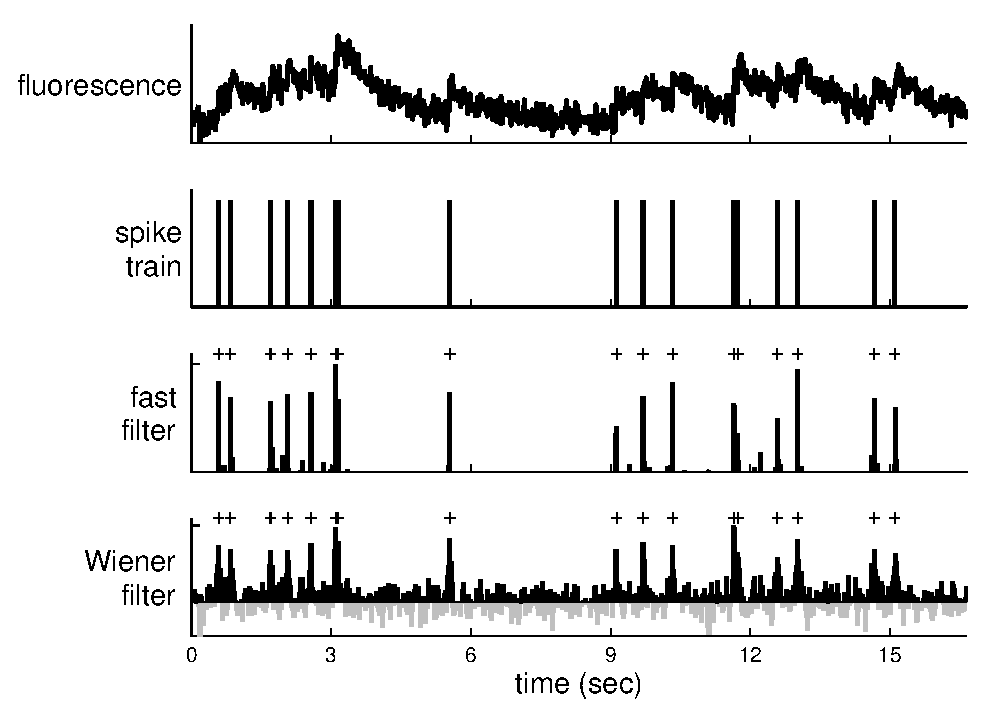
\includegraphics[width=.9\linewidth]{/Users/joshyv/Research/oopsi/fast-oopsi/figs/woopsi_inf}
\caption[\foopsi filter outperforms Wiener filter]{The \foopsi filter significantly outperforms the optimal linear deconvolution (aka, Wiener) filter on typical simulated data-sets. Top panel: fluorescence trace.  Second panel: spike train.  Third panel: \foopsi filter inference.  Bottom panel: Wiener filter inference.  Gray '$+$'s in bottom two panels indicate true spike times.  Simulation details: $T=2930$ time steps, $\Del=5$ msec, $\alpha=1$, $\beta=0$, $\sig=0.3$, $\tau=1$ sec, $\lam=1$ Hz.} \label{fig:woopsi_inf}
\end{figure}


In the above, the model parameters were assumed to be known.  However, in the general case, the parameters are unknown, and must therefore be estimated from the data.  Section \ref{sec:learn} describes how the parameters of the model may be estimated directly from the observations.  Importantly, this obviates the need to conduct joint imaging and electrophyiological experiments to obtain ``training'' data, as the developed approach is fully unsupervised.  Figure \ref{fig:woopsi_learn} shows another simulated example; in this example, however, the parameters are estimated from the observed fluorescence trace.  Again, it is clear that the \foopsi filter far outperforms the Wiener filter.

\begin{figure}[h!]
\centering 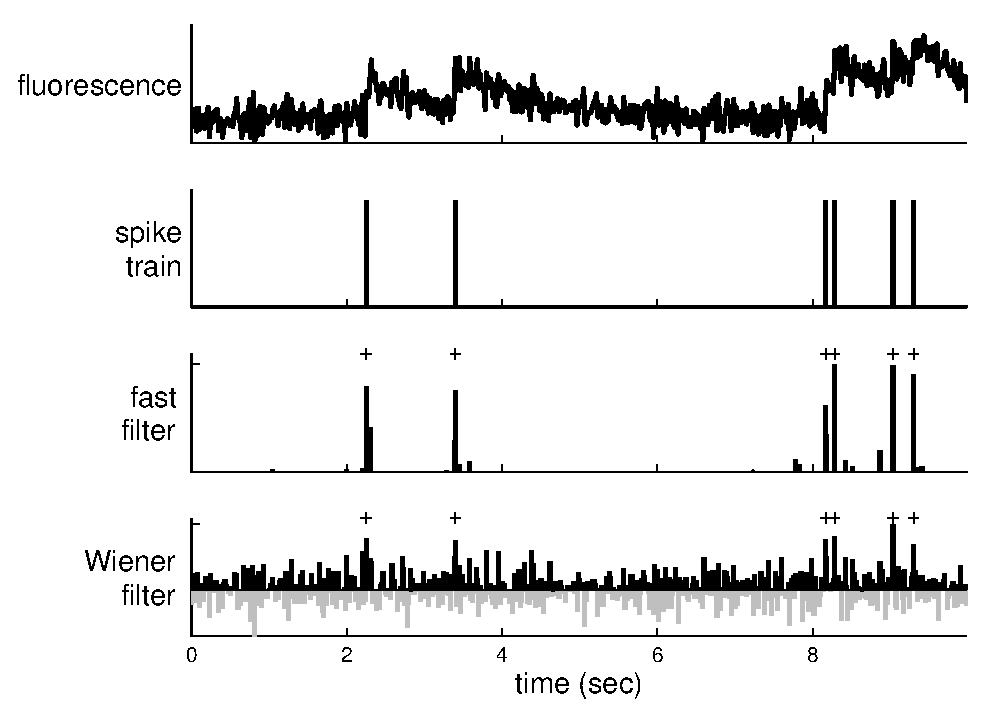
\includegraphics[width=.9\linewidth]{/Users/joshyv/Research/oopsi/fast-oopsi/figs/woopsi_learn}
\caption[parameters may be estimated using the \foopsi filter]{The \foopsi filter significantly outperforms the Wiener filter, even when estimating the parameters only from the observed data.  Simulated details as in Figure \ref{fig:woopsi_inf}.} \label{fig:woopsi_learn}
\end{figure}

Given the above two results, the \foopsi filter was applied to real data.  More specifically, by simultaneously recording electrophysiologically and imaging, the true spike times are known, and the accuracy of the two filters can be compared.  Figure \ref{fig:woopsi_data} shows similar result for this typical in vitro data-set.  These results are typical of the 12 joint electrophysiological and imaging experiments conducted (not shown). Note that the first few ``events'' are actually pairs of spikes, which is reflected in the inferred spike trains.

\begin{figure}[h!]
\centering 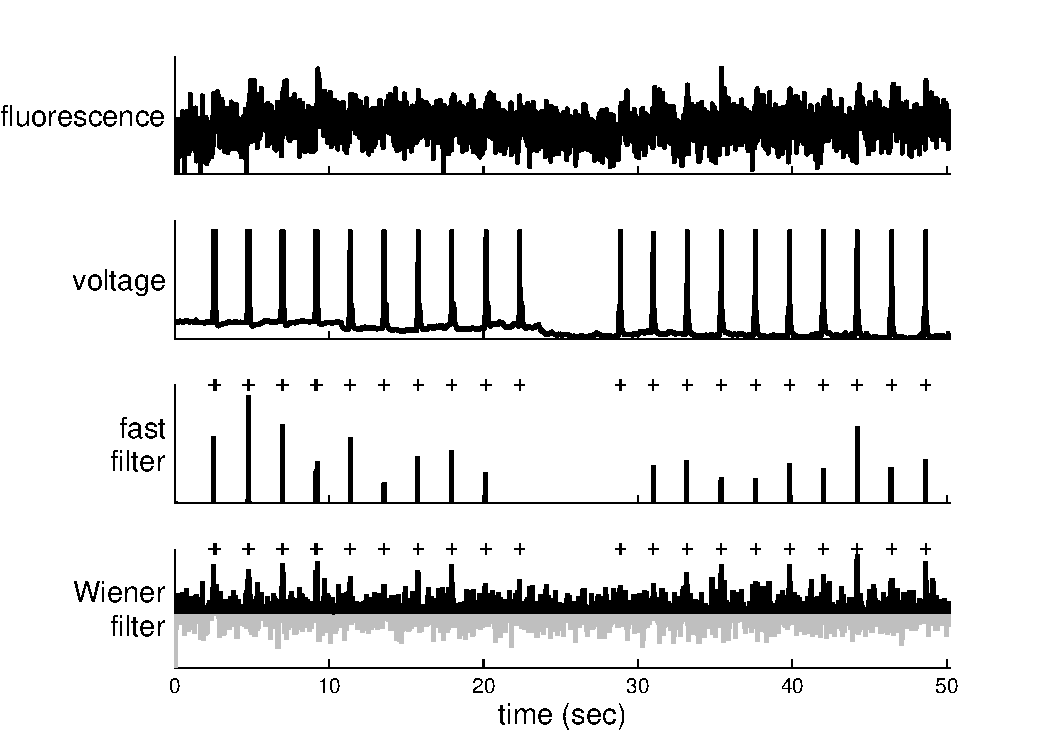
\includegraphics[width=.9\linewidth]{/Users/joshyv/Research/oopsi/fast-oopsi/figs/woopsi_data4}
\caption[\foopsi filter outperforms Wiener filter on real data]{The \foopsi filter significantly outperforms the Wiener filter on typical in vitro data-sets.  Note that all the parameters for both filters were estimated from the data.} \label{fig:woopsi_data}
\end{figure}

\subsection{Online analysis of spike trains using the \foopsi filter}

A central aim for this work was the development of a algorithm that infers spikes sufficiently efficiently to use online while imaging a large population (eg, $\approx 100$) of neurons.  Figure \ref{fig:pop} shows the result of running \foopsi on 136 neurons, recorded simultaneously, as described in the Methods section.  Note that the filtered fluorescence signals much more clearly show fluctuations in spiking. These spike trains were inferred in approximately real time, meaning that one could infer spike trains for the past experiment while conducting the subsequent experiment.


\begin{figure}[h!]
\centering 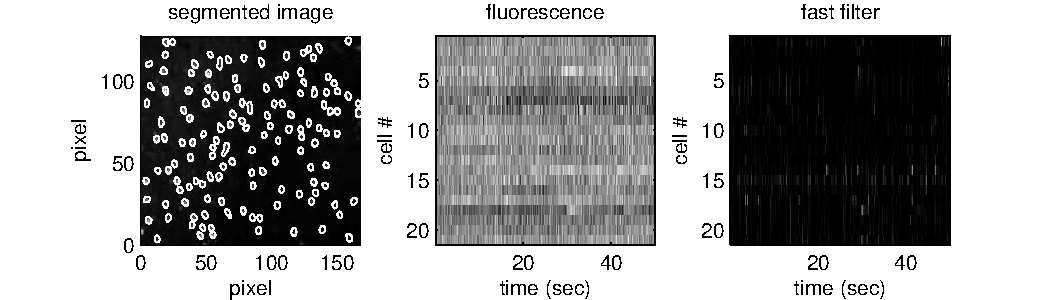
\includegraphics[width=.9\linewidth]{/Users/joshyv/Research/oopsi/fast-oopsi/figs/pop}
\caption[\foopsi filter is robust and works online for populations of neurons]{Applying the \foopsi filter in real time to a large population of neurons imaged simultaneously.  The inferred spike trains convey much more clearly the neural activity.  Left panel: Mean segmented image field.  Middle panel: example fluorescence traces.  Right panel: \foopsi filter output corresponding to each associated trace.} \label{fig:pop}
\end{figure}


\subsection{Extensions}

Section \ref{sec:model} describes a simple principled first-order model relating the spike trains to the fluorescence trace. A number of the simplifying assumptions can be straightforwardly relaxed, including: (i) the Gaussianity of the noise on the fluorescence measurements, and (ii) the static nature of the prior, $\lam$.  Combining these two modifications into the model yields:


\begin{align}
	F_t &\sim \text{Poisson}(\alpha C_t + \beta) \label{eq:nonlin} \\
	% C_t &= (1-\Del/\tau)C_{t-1} + n_t
	n_t &\sim \text{Poisson}(\lam_t \Del),
\end{align}

\noindent where the dynamics for calcium are as before.  To modify the \foopsi filter to be optimal for this new model, the gradient and Hessian of this new model can be analytically computed.  Note that both the above assumptions maintain the log-concavity of the posterior, meaning that by using Newton-Raphson, obtaining the globally optimal solution is still guaranteed. Unfortunately, inference did not improve when using this new model, for either in silico or in vitro experiments (not shown).

Often, the as intracellular calcium accumulates, the fluorescence signal begins to saturate \cite{PologrutoSvoboda04}.  This observation may be incorporated into the model quite easily:

\begin{align}
	F_t &= \alpha \frac{C_t}{C_t+k_d} + \beta +  \sig \varepsilon_t, \qquad \varepsilon_t \overset{iid}{\sim} \mN(0,1).
\end{align}

\noindent where $C_t/(C_t+k_d)$ is the standard Hill equation \cite{PologrutoSvoboda04}.  Incorporating this nonlinearity breaks the log-concavity of the posterior, meaning that converging to the global maximum is no longer guaranteed.  Assuming a good initialization can be found, however, if this model is more accurate, than ascending the gradient for this model might yield improved inference results.  In practice, initializing with the linear solution often resulted in approximately equally good inference, but this nonlinear inference was far less robust than the inference assuming the linear model (not shown).  
%Unfortunately, using this more powerful model did not result in substantial inference improvements for simulated or in vitro data (not shown).  This is possibly due to approximating the Poisson distribution governing spiking with an exponential distribution.  This approximation is required to ensure concavity of the posterior.  

A previously proposed sequential Monte Carlo (SMC) method to infer spike trains \cite{VogelsteinPaninski09} can incorporate this nonlinearity, as well as the other model extensions, more elegantly. However, this SMC filter is not nearly as efficient as the fast filter proposed here.  Like the fast filter, the SMC filter estimates the model parameters in a completely unsupervised fashion, ie, from the fluorescence observations, using an expectation-maximization algorithm.  In \cite{VogelsteinPaninski09}, parameters for the SMC filter were initialized based on other data-sets.  While effective, this initialization was often far from the final estimates, and therefore, required a relatively large number of iterations (eg, 20-25) before converging.  Thus, it seemed that the \foopsi filter could be used to obtain an improvement to the initial parameter estimates, reducing the required number of iterations.  Indeed, Figure \ref{fig:smc_init} shows how the SMC filter outperforms the \foopsi filter on in vitro data, and only required $3$--$5$ iterations to converge.  Note that the first few events are individual spikes, resulting in relatively small fluorescence fluctuations, whereas the next events are actually spike doublets, causing a much larger fluorescence fluctuation.  Only the SMC filter picks up the individual spikes in this trace, a result typical when the effective signal-to-noise ratio (SNR) is so poor.  Thus, these two inference algorithms are complementary: the \foopsi filter can be used for rapid, online inference, and for initializing the SMC filter, which can then be used to further refine the spike train estimate.

\begin{figure}[h!]
\centering 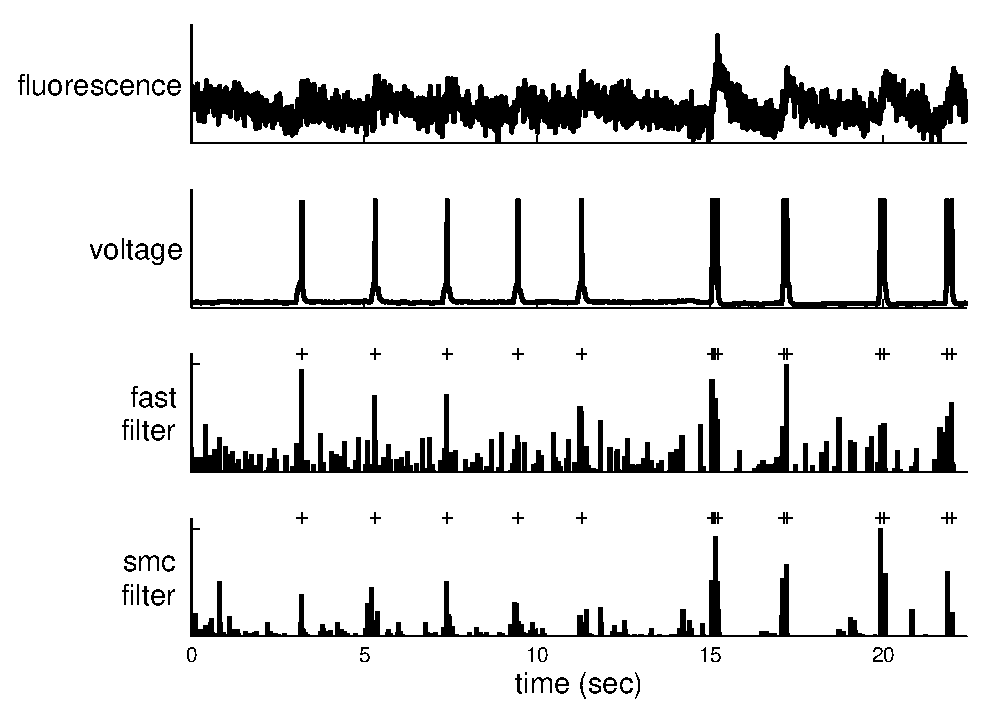
\includegraphics[width=.9\linewidth]{/Users/joshyv/Research/oopsi/fast-oopsi/figs/smc_init12}
\caption[\foopsi filter can initialize Wiener filter]{The \foopsi filter effectively initializes the parameters for the SMC filter (which outperforms the \foopsi filter), significantly reducing the number of expectation-maximization iterations to convergence.  Note that the ordinate on the bottom panel corresponds to the probability of a spike having occurred in each frame.} \label{fig:smc_init}
\end{figure}

\subsection{Spatial filter}

In the above, the data was assumed to be one-dimensional fluorescence traces.  In actuality, the data is a time series of images, which are first segmented into regions-of-interest (ROI), and typically, then averaged, to obtain $F_t$.  In theory, one could improve the effective SNR of the fluorescence trace by scaling each pixel relative to one another.  In particular, pixels not containing any information about calcium fluctuations can be ignored, and pixels that are approximately anti-correlated with one another could have weights with opposing signs.  

Figure \ref{fig:spatial} demonstrates the potential utility of this approach.  The top row shows different depictions of an ROI containing a single neuron.  On the far left panel is the true spatial filter for this neuron.  This particular spatial filter was chosen based on experience analyzing both in vitro and in vivo movies; often, it seems that the pixels immediately around the soma are anti-correlated with those in the soma.  This effect is possibly due to the influx of calcium from extracellular space immediately around the soma.  This simulated movie is relatively noisy, as indicated by the second panel, which depicts an exemplary image frame.  The standard approach, given such a noisy movie, would be to first segment the movie to find an ROI corresponding to the soma of this cell, and then spatially average all the pixels found to be within this ROI.  The third panel shows this ``typical spatial filter''.  The forth panel shows the mean frame, ie, $\langle \vbF \rangle_t$.  Clearly, this mean frame is very similar to the true spatial filter.

The bottom panels of Figure \ref{fig:spatial} depict the effect of using the true spatial filter, versus the typical one. The left side shows the fluorescence trace and its associated spike inference obtained from using the typical spatial filter.  The right side shows the same when using the true spatial filter.  Clearly, the true spatial filter results in a much cleaner fluorescence trace and spike inference.  


\begin{figure}[h!]
\centering 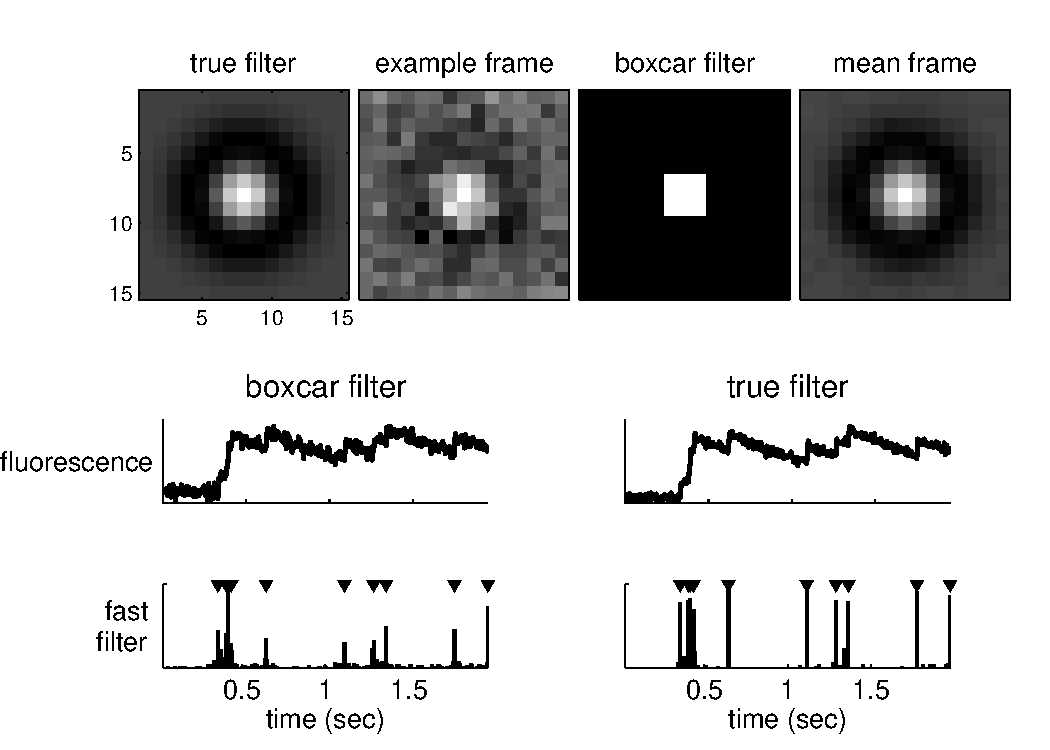
\includegraphics[width=.9\linewidth]{/Users/joshyv/Research/oopsi/fast-oopsi/figs/spatial2}
\caption[spatial filtering can improve effective SNR]{A simulation demonstrating that using a better spatial filter can significantly enhance the effective SNR (see Supplementary Movie 1 for the full movie associated with this simulation). The true spatial filter was a sum of Gaussians: a positively weighted small variance Gaussian, and a negatively weighted large variance Gaussian (both with the same mean).  Top row far left: true spatial filter.  Top row second from left: example frame (frame number 100). Top row second from right: typical spatial filter.   Top row far right: mean frame.  Middle row left: fluorescence trace using typical spatial filter. Bottom row left: \foopsi filter output using typical spatial filter.  Middle row right: fluorescence trace using true spatial filter.  Bottom right: \foopsi filter output using true spatial filter. Simulation details: $\valpha=\mN(\ve{0},2 \bI)-1.1 \mN(\ve{0},2.5 \bI)$ where $\mN(\ve{mu},\ve{\Sig})$ indicates a Gaussian with mean $\ve{\mu}$ and covariance matrix $\ve{\Sig}$, $\bbeta=1$, $\tau=0.85$ sec, $\lam=5$ Hz.} \label{fig:spatial} 
\end{figure}



\subsection{Overlapping spatial filters}


The above shows that if a ROI contains only a single neuron, the effective SNR can be enhanced by spatially filtering.  However, this analysis assumes that only a single neuron is in the ROI.  Often, neural spatial filters are overlapping, or nearly overlapping, making the segmentation problem even more difficult.  Therefore, it is desirable to have an ability to crudely segment, yielding only a few neurons in each ROI, and then spatially filtering within each ROI to pick out the spike trains from each neuron.  This may be achieved in a principled manner by generalizing the model as described in Section \ref{sec:methods:overlapping}.  Figure \ref{fig:spatial_multi_inf} shows an example of this approach on simulated data. Note that the spatial filters are sufficiently overlapping that some ``bleed-though'' can be seen across the traces.  


\begin{figure}[h!]
\centering 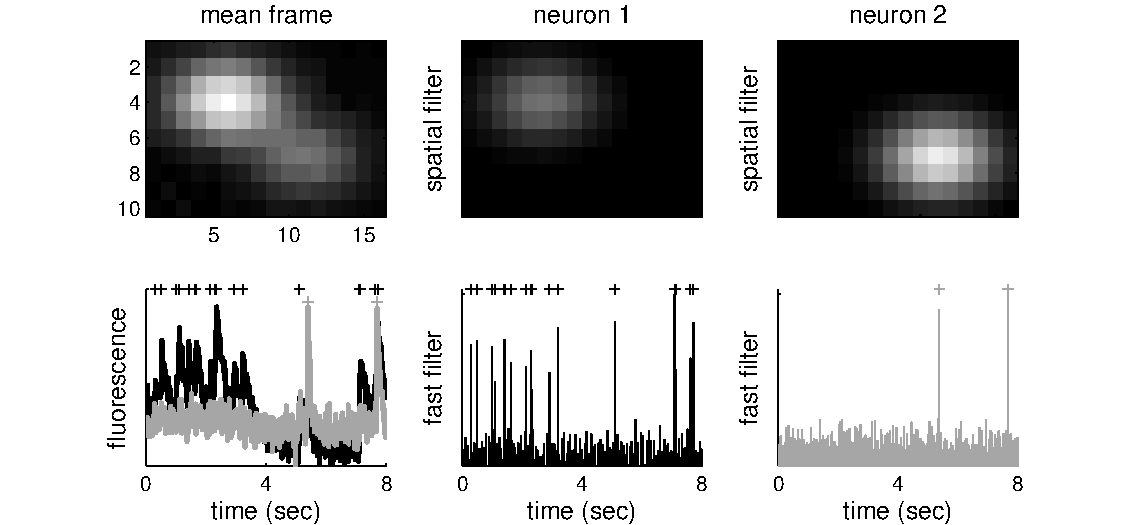
\includegraphics[width=.9\linewidth]{/Users/joshyv/Research/oopsi/fast-oopsi/figs/spatial_multi_inf}
\caption[overlapping spatial filters are not problematic]{Simulation showing that even when two neurons' spatial filters are overlapping, one can separate the two signals by spatial filtering. Simulation details: $\valpha^1=\mN([-1.8 1.8],2 \bI)\, \valpha^2=\mN([1.8 -1.8],5 \bI)$, $\bbeta=[1 1]\T$, $\tau=[0.5 0.5]\T$ sec, $\lam=[1.5 1.5]$ Hz.} \label{fig:spatial_multi_inf}
\end{figure}

While Figure \ref{fig:spatial_multi_inf} shows that one could separate the signals if the spatial filters of the neurons were known, Figure \ref{fig:spatial_multi_learn} shows that the spatial filters can be estimated using only the fluorescence movie, by using the approach described in Section \ref{sec:methods:overlapping}.


\begin{figure}[h!]
\centering 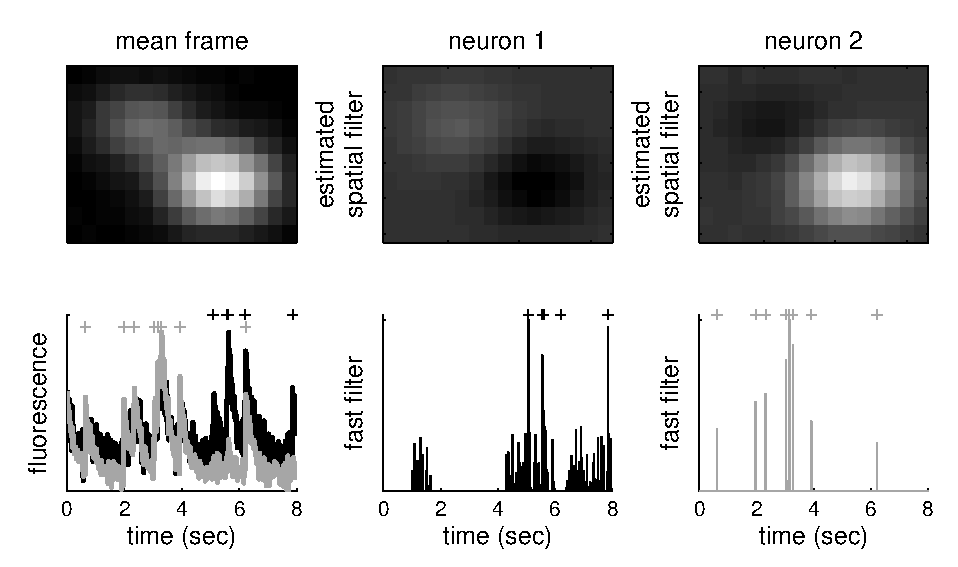
\includegraphics[width=.9\linewidth]{/Users/joshyv/Research/oopsi/fast-oopsi/figs/spatial_multi_learn}
\caption[overlapping spatial filters can be estimated]{Simulation showing that even when two neuron's spatial filters are largely overlapping, the spatial filter of each can be inferred, to separate the two signals. Simulation details as above.} \label{fig:spatial_multi_learn}
\end{figure}





\section{Discussion} \label{sec:dis}

% \paragraph{Summary}

Above, an algorithm to approximate the \emph{maximum a posteriori} (MAP) spike train, given a fluorescence trace was developed.  The approximation is required because finding the actual MAP estimate is not currently computationally tractable.  Replacing the assumed Poisson distribution on spikes with an exponential distribution yields a log-concave optimization problem, which can be solved using standard gradient ascent techniques (such as Newton-Raphson).  This exponential distribution has an advantage over a Gaussian distribution by restricting spikes to be positive, which improves inference quality (c.f. Figure \ref{fig:woopsi_inf}).  This result is common within machine learning \cite{Hoyer04,OGradyPearlmutter06}: imposing a non-negative constraint often helps prevent oscillations and other overfitting artifacts. This non-negative constraint is enforced by interior-point methods.  Furthermore, by utilizing the special structure of the Hessian matrix (ie, it is tridiagonal), this approximate MAP spike train can be found.  Importantly, this algorithm runs fast enough on standard computers that it can be run online.  Finally, all the parameters can be estimated from only the fluorescence observations, obviating the need for joint electrophysiology and imaging (c.f. Figure \ref{fig:woopsi_learn}).  This approach is robust, in that it works ``out-of-the-box'' on all the in vivo and in vitro data analyzed (c.f. Figure \ref{fig:woopsi_data}).

This work is closely related to several previously proposed algorithms.  Ideally, one could compute the full joint posterior of entire spike trains, conditioned on the fluorescence data.  This distribution is analytically intractable, due to the Poisson assumption on spike trains.  A Bayesian approach could use Markov Chain Monte Carlo to recursively sample spikes until a whole sample spike train is obtained \cite{AndrieuDoucet01}.  Because a central aim here was computational expediency, a ``greedy'' approach is natural: ie, recursively sample the most likely spike, update the posterior, and repeat until the posterior stops increasing.  Template matching, projection pursuit regression \cite{FS81}, and matching pursuit \cite{MallatZhang93} are examples of such a greedy approach (Greenberg et al's algorithm could also be considered a special case of such a greedy approach).  Both the greedy methods, and the one developed here, aim to optimize a similar objective function.  While greedy methods reduce the computational burden by restricting the search space of spike trains, here analytic approximations are made.  The advantage of the greedy approaches relative to this one is that they result in a spike train (ie, a binary sequence), whereas the approach developed herein is faster, and guaranteed to be optimal, given the approximations.  


Because this filter is model based, it can generalized in several ways to improve accuracy.  Unfortunately, some of these generalizations do not improve inference accuracy, probably because of the exponential approximation.  Instead, the \foopsi filter output can be used to initialize the SMC filter \cite{VogelsteinPaninski09}, to further improve inference quality (c.f. Figure \ref{fig:smc_init}).  Another model generalization allows incorporation of spatial filtering of the raw movie into this approach (c.f. Figure \ref{fig:spatial}).  The parameters of the spatial filter can be estimated from the data, even when spatial filters are overlapping (c.f. Figure \ref{fig:spatial_multi_learn}).

A number of extensions follow from this work.  First, further development on some of the model generalizations may improve inference results. Second, putting this filter with a crude but automatic segmentation tool to obtain ROIs would create a completely automatic algorithm that converts raw movies of populations of neurons into populations of spike trains.  Third, combining this algorithm with recently developed connectivity inference algorithms on this kind of data \cite{MishchenkoPaninski09}, could yield very efficient connectivity inference.